% !TEX program = xelatex
% BitDA 期末專題 — 題目 A：各種 AMM 機制比較研究
% 編譯流程：xelatex -> bibtex -> xelatex -> xelatex
\documentclass[11pt,a4paper]{article}

% ---------- 字型與中文 ----------
\usepackage{fontspec}
\usepackage{xeCJK}
\setCJKmainfont[AutoFakeSlant=0.2]{PingFang TC}
\setCJKsansfont{PingFang TC}
\setCJKmonofont{PingFang TC}
\XeTeXlinebreaklocale "zh"
\XeTeXlinebreakskip = 0pt plus 1pt

% ---------- 版面 ----------
\usepackage[a4paper,margin=2.4cm]{geometry}
\usepackage{amsmath,amssymb,mathtools}
\usepackage{graphicx}
\usepackage{booktabs}
\usepackage{tabularx}
\usepackage{array}
\usepackage{float}
\usepackage{caption}
\usepackage{subcaption}
\usepackage{xcolor}
\usepackage{microtype}
\usepackage{fancyhdr}
\usepackage[numbers,sort&compress]{natbib}
\usepackage{tikz}
\usetikzlibrary{arrows.meta,positioning,calc}
\usepackage[colorlinks=true,linkcolor=blue!55!black,citecolor=teal!60!black,urlcolor=magenta!60!black]{hyperref}

\captionsetup{font=small,labelfont=bf}
\setlength{\parskip}{0.45em}
\renewcommand{\arraystretch}{1.25}

% 頁首頁尾
\pagestyle{fancy}
\fancyhf{}
\rhead{\small 各種 AMM 機制比較研究}
\lhead{\small BitDA 期末專題 — 題目 A}
\cfoot{\thepage}
\renewcommand{\headrulewidth}{0.4pt}

% 重點框
\newcommand{\keybox}[1]{%
  \par\smallskip\noindent
  \fcolorbox{black!25}{blue!5}{%
    \begin{minipage}{0.975\linewidth}\small\textbf{重點：}\,#1\end{minipage}}%
  \par\smallskip}

% 常用數學縮寫
\newcommand{\IL}{\mathrm{IL}}
\newcommand{\df}{\,\mathrm{d}}

\title{\textbf{各種 AMM 機制比較研究}\\[4pt]
\large Constant-Product、Stable-Swap 與 Weighted-Pool 的數學模型、滑點、無常損失與情境模擬}
\author{BitDA 區塊鏈期末專題 \quad（題目 A）\\[2pt]
\small 姓名：廖振翔\quad 學號：B11705058}
\date{2026 年 6 月}

\begin{document}
\maketitle
\thispagestyle{fancy}

\begin{abstract}\noindent
自動造市商（Automated Market Maker, AMM）是去中心化交易所（DEX）的核心。本報告系統性比較三大 AMM 家族：以
\textbf{Constant-Product}（Uniswap V2/V3）、\textbf{Stable-Swap}（Curve）與
\textbf{Weighted-Pool}（Balancer）為代表。我們首先在
\emph{Constant-Function Market Maker}（CFMM）的統一框架下，逐一推導三者的不變量（invariant）、邊際價格、成交公式與手續費機制；接著從理論與
\textbf{數值模擬}兩個層面，量化比較三者在\textbf{滑點（slippage）、流動性提供者（LP）收益與無常損失（impermanent loss）}上的差異。
我們導出一條貫穿全文的統一規則
$\text{slippage}\approx \Delta x/(2\mathcal{D})$，其中等效深度 $\mathcal{D}$ 分別由準備金 $R$（V2）、$A\cdot R$（Curve 近錨點）、區間內集中流動性 $L$（V3）與權重比 $(W_i/W_o)R$（Balancer）決定，從而以單一視角解釋四種機制的滑點曲線。
在收益面，我們以
\emph{Loss-Versus-Rebalancing}（LVR）理論補充傳統無常損失分析，並用蒙地卡羅（Monte Carlo）模擬在
不同年化波動率（30\%/80\%/150\%）與交易量（10$\times$/50$\times$/200$\times$ TVL）情境下、LP 相對於 HODL 的報酬分佈。
模擬顯示：低波動高量時 Uniswap V3 因集中流動性而報酬最高，但高波動時其無常損失被放大且易跌出區間而表現最差；Balancer 98/2 池最接近 HODL；
手續費收入必須超越無常損失，LP 才能勝過持有。最後以 Uniswap v4 hooks、LVR/MEV 緩解型 AMM（FM-AMM、CoW AMM、am-AMM）與真實 TVL 規模等前沿議題作結。
所有公式皆對照一手白皮書與學術論文驗證，圖表與模擬程式碼可完全重現。
\end{abstract}

{\small\tableofcontents}
\bigskip

% =====================================================================
\section{緒論}
% =====================================================================
傳統中心化交易所（CEX）以\textbf{限價訂單簿（order book）}撮合買賣雙方；造市者持續掛單以提供流動性，價格由買賣盤的最佳報價決定。
然而訂單簿在區塊鏈上維護成本極高（每次掛單／撤單都是一筆交易），且需要專業造市者。
\textbf{自動造市商（AMM）}以一條確定性的數學曲線取代訂單簿：任何人都能把資產存入\emph{流動性池（liquidity pool）}成為被動的流動性提供者（LP），
而交易價格由池中準備金（reserves）透過一個\textbf{不變量函數（invariant）}自動決定。這個轉變使「人人皆可造市」成為可能，也催生了 Uniswap、Curve、Balancer 等協議。

三大 AMM 家族在「\emph{該用哪一條曲線}」上做出不同取捨：
\begin{itemize}
  \item \textbf{Constant-Product}（Uniswap V2 的 $xy=k$）：對任意價格都提供流動性，通用但滑點較大；V3 進一步允許把流動性\emph{集中}到指定價格區間以提升資本效率。
  \item \textbf{Stable-Swap}（Curve）：為\emph{互相錨定}的資產（穩定幣、LST）設計，在錨點附近近乎零滑點。
  \item \textbf{Weighted-Pool}（Balancer）：把兩資產等權的 $xy=k$ 推廣為 $N$ 資產、任意權重的幾何平均造市商，可當作自我再平衡的指數基金。
\end{itemize}

\paragraph{本報告的貢獻與結構。}
本報告同時滿足題目三項要求：\textbf{(1)} 第 2--5 節分析三種 AMM 的\emph{數學模型與核心機制}；
\textbf{(2)} 第 8 節以蒙地卡羅\emph{模擬不同流動性與交易量情境}；
\textbf{(3)} 第 6--8 節\emph{視覺化滑點、LP 收益與無常損失差異}（共 8 張以 Python 計算之圖表）。
第 9 節給出綜合比較矩陣與選型指南，第 10 節作為額外內容涵蓋 Uniswap v4、LVR/MEV 緩解設計與真實市場規模。

% =====================================================================
\section{統一框架：Constant-Function Market Makers (CFMM)}\label{sec:cfmm}
% =====================================================================
三種 AMM 都屬於\textbf{Constant-Function Market Maker（CFMM）}。一個持有準備金向量 $\mathbf{R}=(R_1,\dots,R_n)$ 的 CFMM 由一個\emph{交易函數} $\varphi(\mathbf{R})$ 定義，
規定一筆交易合法（admissible）的條件是交易後 $\varphi$ 不下降 \citep{angeris2019uniswap,angeris2020oracles}：
\begin{equation}
\varphi(\mathbf{R}_{\text{after}}) \;\geq\; \varphi(\mathbf{R}_{\text{before}}).
\end{equation}
手續費的本質就是讓 $\varphi$ 嚴格上升，差額累積給 LP。對雙資產池 $(x,y)$，三家的交易函數分別為
\begin{equation}
\underbrace{\varphi=xy}_{\text{Uniswap}},\qquad
\underbrace{\varphi=x^{w_x}y^{w_y},\ w_x+w_y=1}_{\text{Balancer}},\qquad
\underbrace{An^n(x{+}y)+D-\tfrac{D^{n+1}}{n^n xy}}_{\text{Curve StableSwap}}.
\end{equation}
對任一光滑不變量，\textbf{邊際價格（marginal/spot price）}是不變量曲線的斜率：把 $\varphi(x,y)=\text{const}$ 全微分得
$p \equiv -\dfrac{\df y}{\df x} = \dfrac{\partial\varphi/\partial x}{\partial\varphi/\partial y}$。
有限大小的交易會沿曲線移動，使\emph{實際成交均價}劣於邊際價格，兩者之差即\textbf{滑點}。手續費 $1-\gamma$ 則在邊際價格周圍張開一條
$\gamma : 1/\gamma$ 的無套利價帶（no-arbitrage band），對應 AMM 的買賣價差 \citep{angeris2019uniswap}。

\keybox{三種 AMM 本質相同——都是 CFMM，差別\emph{只}在交易函數 $\varphi$ 的選擇。$\varphi$ 的\emph{曲率}決定滑點，$\varphi$ 的\emph{形狀}決定無常損失。後續各節即是在比較不同 $\varphi$ 帶來的取捨。}

圖~\ref{fig:bonding} 把三者畫在同一張準備金平面上：constant-sum（$x+y=D$，零滑點但無法承受價格偏離錨點）與 constant-product（$xy=k$）是兩個極端，
StableSwap 透過放大係數 $A$ 在兩者間連續插值，Balancer 80/20 則是一條不對稱的幾何平均曲線。

\begin{figure}[H]
\centering
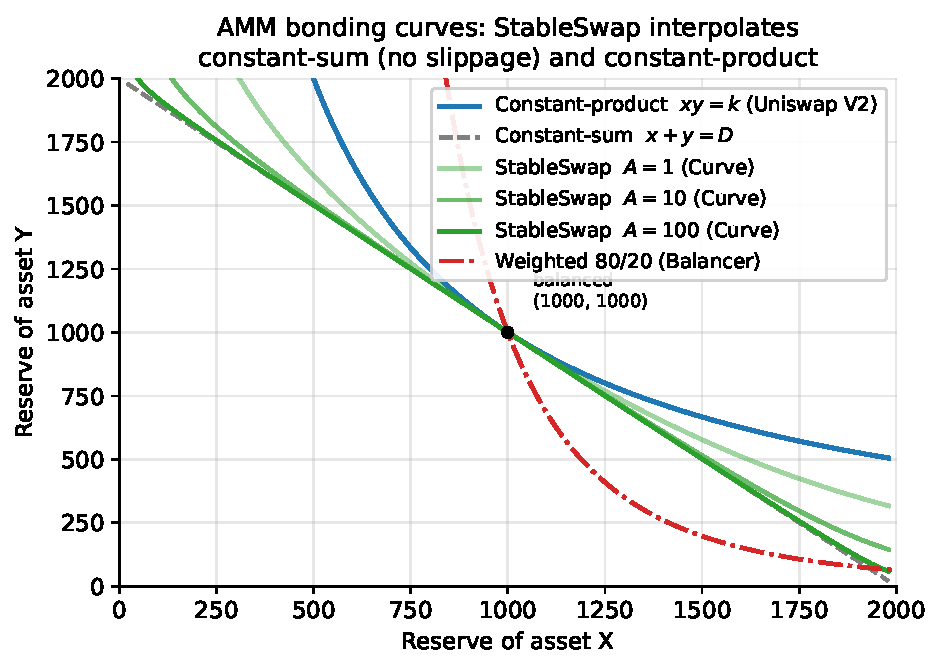
\includegraphics[width=0.74\linewidth]{figures/fig_bonding_curves.pdf}
\caption{三大 AMM 的鍵結曲線（bonding curve）。所有曲線通過平衡點 $(1000,1000)$。StableSwap 的放大係數 $A$ 越大，曲線在錨點附近越貼合 constant-sum（近零滑點），在極端處才彎向 constant-product。}
\label{fig:bonding}
\end{figure}

% =====================================================================
\section{Constant-Product 機制：Uniswap V2 與 V3}
% =====================================================================
\subsection{Uniswap V2：\texorpdfstring{$x\cdot y=k$}{xy=k}}
Uniswap V2 \citep{uniswapv2wp} 是最典型的 constant-product market maker。每個交易對合約持有兩種 ERC-20 代幣準備金 $x,y$，並強制不變量
\begin{equation}
x\cdot y = k .
\end{equation}
手續費（預設 0.3\%，$30$ basis points）課在\emph{輸入}金額上，保留比例 $\gamma=997/1000=0.997$。輸入 $\Delta x$ 的代幣 X、得到的 Y 為
\begin{equation}\label{eq:v2swap}
\Delta y \;=\; \frac{997\,y\,\Delta x}{1000\,x+997\,\Delta x}
\;=\; \frac{(1-\phi)\,y\,\Delta x}{x+(1-\phi)\,\Delta x},\qquad \phi=0.003 .
\end{equation}
這等價於要求 $(x+0.997\Delta x)(y-\Delta y)=xy$：只有 $99.7\%$ 的輸入被計入曲線，但全額進入準備金，使 $k$ 嚴格成長、$0.3\%$ 累積給 LP。
鏈上實際檢查的是手續費調整後不變量 $(x_1-0.003\,x_{\text{in}})\,y_1 \ge x_0 y_0$（白皮書式 9）\citep{uniswapv2wp,uniswapv2docs}。

\textbf{邊際與實際價格。} 忽略手續費時邊際價格 $p=y/x$（無窮小交易的極限價）。有限交易的實際均價
$\bar p=\Delta y/\Delta x = 997\,y/(1000x+997\Delta x)$ 永遠劣於 $p$。以輸入佔準備金比例 $f=\Delta x/x$ 表示（免手續費）：
\begin{equation}\label{eq:v2impact}
\bar p = \frac{y}{x}\cdot\frac{1}{1+f},\qquad
\frac{p_{\text{new}}}{p_{\text{old}}}=\frac{1}{(1+f)^2}=1-2f+3f^2-4f^3+\cdots
\end{equation}
故滑點對小額交易\emph{近似線性}成長、對大額交易轉為\emph{凸（超線性）}，且 $f\to\infty$ 時價格衝擊發散——池子\emph{永遠無法被抽乾}。
在無套利下，Uniswap 價格被夾在 $\gamma\,m_p \le y/x \le m_p/\gamma$（$m_p$ 為外部參考價）\citep{angeris2019uniswap}。

\textbf{無常損失（Impermanent Loss）。} 當外部價格比變為 $r=P'/P$，50/50 池因沿 $xy=k$ 自動「賣漲買跌」而再平衡，產生相對於持有的損失：
\begin{equation}\label{eq:v2il}
\IL(r)=\frac{V_{\text{pool}}}{V_{\text{hold}}}-1=\frac{2\sqrt{r}}{1+r}-1\;\le\;0,
\end{equation}
其中 $V_{\text{hold}}=y_0+x_0P'$、$V_{\text{pool}}=2\sqrt{kP'}$。由 AM--GM 不等式可知 $\IL\le 0$，且對 $r\leftrightarrow 1/r$ 對稱：$r=2$（或 $0.5$）為 $-5.72\%$，$r=4$ 為 $-20\%$。

\textbf{LP 代幣機制。} 首次注入鑄造 $\sqrt{xy}$ 單位流動性代幣（並永久鎖定 $1000$ 單位 MINIMUM\_LIQUIDITY），之後等比例注入鑄造 $s=(\Delta x/x)\cdot\text{totalSupply}$。
手續費\emph{複利}進 $k$（贖回時一併取回），可選的協議費（feeTo）抽取 LP 費的 $1/6$ \citep{uniswapv2wp}。

\subsection{Uniswap V3：集中流動性（Concentrated Liquidity）}
Uniswap V3 \citep{uniswapv3wp} 讓每個 LP 把流動性\emph{集中}於任意價格區間 $[p_a,p_b]$，而非分散在 $(0,\infty)$。在區間\emph{內}，部位行為等同一個運作於\textbf{虛擬準備金}的 V2 池：
\begin{equation}
L^2=x\cdot y\quad(\text{虛擬}),\qquad
\Bigl(x_{\text{real}}+\tfrac{L}{\sqrt{p_b}}\Bigr)\Bigl(y_{\text{real}}+L\sqrt{p_a}\Bigr)=L^2 .
\end{equation}
其中流動性 $L$ 滿足關鍵線性關係 $L=\Delta y/\Delta\sqrt{P}$，使換算數學線性化。價格 $P$ 在區間內時的真實持倉為
\begin{equation}\label{eq:v3reserves}
x=L\!\left(\frac{1}{\sqrt{P}}-\frac{1}{\sqrt{p_b}}\right),\qquad
y=L\!\left(\sqrt{P}-\sqrt{p_a}\right),
\end{equation}
在 $P=p_b$ 時部位全為 Y、$P=p_a$ 時全為 X \citep{elsts2021liquiditymath}。價格空間以\textbf{tick} 離散化：$p(i)=1.0001^{\,i}$（每 tick 為 1 basis point），合約追蹤
$\sqrt{P}$ 與當前 tick $i_c=\lfloor\log_{1.0001}P\rfloor$。手續費分四級 $0.01/0.05/0.30/1\%$（tick spacing 各為 $1/10/60/200$），且\emph{不複利}（以獨立餘額累計，部位多以 ERC-721 NFT 表示）\citep{uniswapfeetiers,uniswapv3concentrated}。

\textbf{資本效率與無常損失放大。} 相對於全區間 V2，集中部位的資本效率倍率為 \citep{adams2021tweet}
\begin{equation}\label{eq:v3eff}
E=\frac{1}{1-\bigl(p_a/p_b\bigr)^{1/4}} .
\end{equation}
區間越窄、$E$ 越大（白皮書指可達約 $4000\times$）。但代價是：在區間內無常損失被\emph{同比例放大}，且一旦價格\emph{跌出區間}，部位全轉為單一資產、停止賺取手續費（變成靜態持有，與 HODL 偏離更遠）；此集中流動性部位的損益可用歐式選擇權靜態複製 \citep{deng2022staticreplication}。
圖~\ref{fig:v3} 量化了這個「資本效率 $\leftrightarrow$ 無常損失」的取捨。

\begin{figure}[H]
\centering
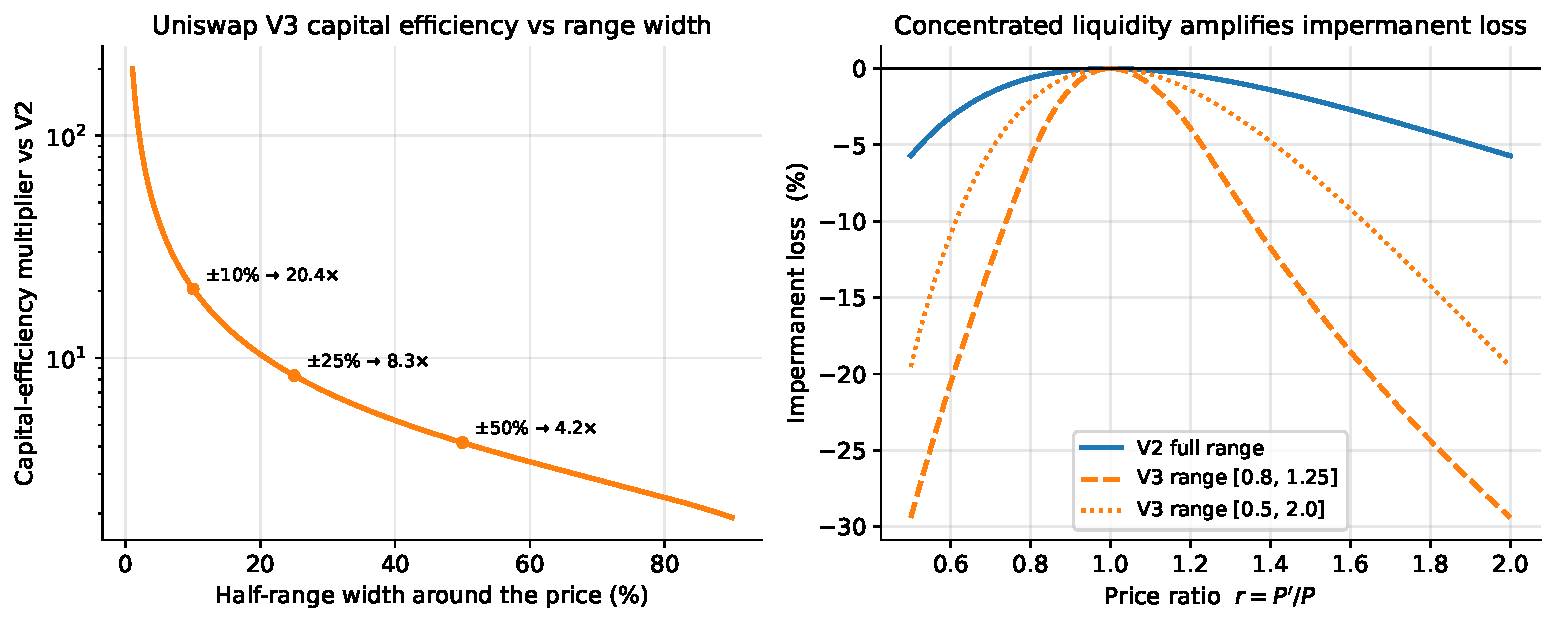
\includegraphics[width=0.97\linewidth]{figures/fig_v3_efficiency.pdf}
\caption{（左）Uniswap V3 資本效率倍率隨價格區間寬度變化：$\pm10\%$ 區間即達約 $20\times$。（右）集中流動性放大無常損失：相同價格變動下，窄區間 V3 的 IL 遠大於全區間 V2。}
\label{fig:v3}
\end{figure}

% =====================================================================
\section{Stable-Swap 機制：Curve}
% =====================================================================
\subsection{StableSwap 不變量與放大係數 \texorpdfstring{$A$}{A}}
Curve 的 StableSwap \citep{egorov2019stableswap,curvewhitepapersdocs} 專為\emph{互相錨定}的資產設計。其精神是在兩個極端不變量之間插值：constant-sum（$\sum_i x_i=\text{const}$，價格恆為 1、零滑點，但無法承受真實價格偏離）與
constant-product（$\prod_i x_i=\text{const}$，永遠提供流動性但滑點大）。Egorov 以一個\emph{動態槓桿} $\chi$ 把兩者結合，得到 $n$ 幣的 StableSwap 不變量：
\begin{equation}\label{eq:stableswap}
\boxed{\;A\,n^{n}\sum_i x_i + D = A\,D\,n^{n} + \frac{D^{\,n+1}}{n^{n}\prod_i x_i}\;}
\qquad\text{其中}\quad \chi=\frac{A\,n^{n}\prod_i x_i}{D^{n}} .
\end{equation}
$\chi$ 在完美平衡（$x_i=D/n$）時等於放大係數 $A$，隨池子失衡而衰減到 0：$\chi\to\infty$ 為 constant-sum、$\chi\to 0$ 為 constant-product。
$D$ 是參數化曲線的不變量，等於平衡時的總存款（$D=n\,x_{\text{eq}}$）；由於不變量對 $D$ 是高次多項式，$D$ 與成交後餘額 $x_j$ 皆以\textbf{牛頓法}（整數運算）求解。

\textbf{滑點行為。} 接近錨點時 $\chi\approx A$ 主導，曲線進入平坦的 constant-sum 區，邊際價格 $\approx 1$、滑點近乎為零——等效深度被放大約 $A$ 倍。
一旦池子嚴重失衡，$\prod_i x_i$ 崩塌、$\chi\to 0$，不變量退化為 constant-product，滑點\emph{急遽上升}（甚至超過 Uniswap，因被抽乾側準備金已很小）。這正是 $A$ 的取捨：以「錨點附近的平坦／深度」換取「脫錨時的尾部風險」。圖~\ref{fig:ssA} 視覺化此現象。

\textbf{無常損失。} 因資產互相錨定、曲線在 1 附近平坦，pegged 資產的無常損失\emph{極小}；只有當錨\emph{真正斷裂}時才顯著，此時 LP 會累積貶值（較便宜）的那一側資產。Egorov 原始 DAI/USDC/USDT 回測得最佳 $A=85$、手續費 $0.06\%$ \citep{egorov2019stableswap}。

\begin{figure}[H]
\centering
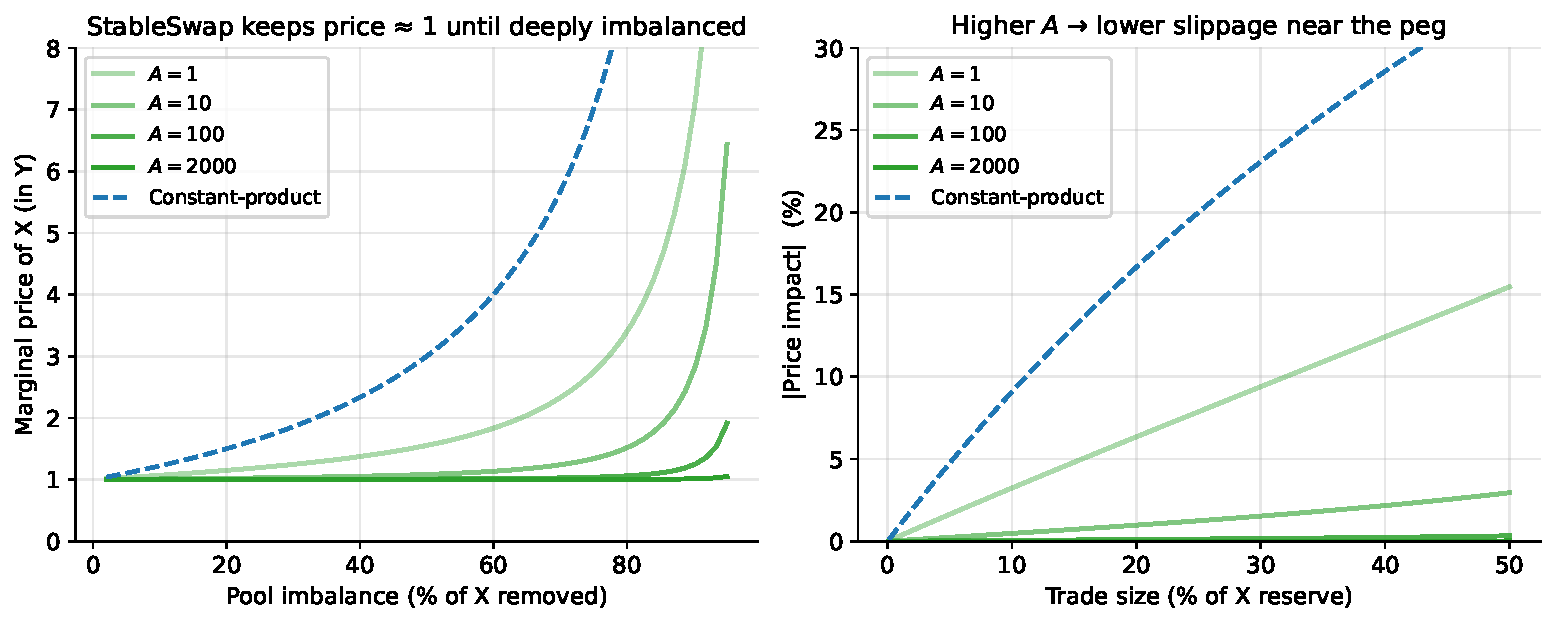
\includegraphics[width=0.97\linewidth]{figures/fig_stableswap_A.pdf}
\caption{放大係數 $A$ 的作用。（左）池子失衡時的邊際價格：$A$ 越大，價格在大幅失衡前都緊貼 1。（右）相同交易量下，$A$ 越大則錨點附近滑點越低；虛線為 constant-product 基準。}
\label{fig:ssA}
\end{figure}

\subsection{Curve V2（CryptoSwap）：動態錨定}
Curve V2 \citep{egorov2021cryptoswap} 把上述設計推廣到\emph{波動、不錨定}的資產（如 ETH/BTC/USD）。它引入轉換後價格空間（透過 \texttt{price\_scale} 向量 $p$ 把真實餘額轉為 $b'_i=b_i/p_i$），
把 StableSwap 式的低滑點區\emph{集中}在當前內部價格附近而非固定的 1.0。其係數改為
\begin{equation}
K=\frac{A\,K_0\,\gamma^{2}}{(\gamma+1-K_0)^{2}},\qquad K_0=\frac{\prod_i x_i\,N^{N}}{D^{N}},
\end{equation}
$\gamma$（典型 $10^{-4}$）控制平坦區寬度。\textbf{動態錨定（repegging）}用一個內部 EMA 價格預言機追蹤市價，且\emph{只在獲利足以覆蓋}時才平移 \texttt{price\_scale}（規則：repeg 造成的損失不得超過已累積利潤的一半），
從而在不需人工管理區間的情況下達到類似 V3 的資本效率（對波動對提供約 $5$--$10\times$ 於 $xy=k$ 的流動性集中度）\citep{curvecryptoswapdocs}。

% =====================================================================
\section{Weighted-Pool 機制：Balancer}
% =====================================================================
Balancer \citep{balancerwp,balancerweightedmath,balancerweightedv2} 把 constant-product 推廣為 $N$ 資產的\textbf{幾何平均造市商（G3M）}。其價值函數（不變量）為
\begin{equation}\label{eq:bal}
V=\prod_t B_t^{\,W_t},\qquad \sum_t W_t=1,
\end{equation}
$B_t$ 為代幣餘額、$W_t$ 為正規化權重。此不變量有一漂亮性質：\emph{每種代幣的價值佔比恆等於其權重} $S_n=W_n$，使池子如同由套利者（而非付費經理人）維持目標權重的\textbf{自我再平衡指數基金}。
輸入代幣 $i$、輸出代幣 $o$ 的邊際價格與成交公式（含手續費 $f$）為
\begin{align}
SP_i^{\,o}&=\frac{B_i/W_i}{B_o/W_o},\label{eq:balsp}\\
A_o&=B_o\!\left[\,1-\Bigl(\frac{B_i}{B_i+(1-f)\,A_i}\Bigr)^{\!W_i/W_o}\right].\label{eq:balout}
\end{align}
只用到兩個被交易代幣的餘額與權重，故 $N$ 幣池中任一對皆可獨立定價。\textbf{Uniswap V2 即是等權 50/50 的特例}：$W_i=W_o=\tfrac12$ 使 \eqref{eq:bal} 退化為 $B_iB_o=k$、\eqref{eq:balout} 退化為 V2 的 $997/1000$ 報價。

\textbf{加權無常損失。} 對任意權重，
\begin{equation}\label{eq:balil}
\frac{V_{\text{pool}}}{V_{\text{hold}}}=\frac{\prod_i (p_i'/p_i)^{\,w_i}}{\sum_i w_i\,(p_i'/p_i)},
\qquad\text{單一資產變動時}\quad \IL(w,r)=\frac{r^{\,w}}{w\,r+(1-w)}-1 .
\end{equation}
把權重集中在會大幅變動的資產上可降低無常損失：對 $2\times$ 變動，50/50 損失 $5.72\%$，80/20 僅 $3.27\%$（少約 $43\%$）；對 $5\times$ 變動，50/50 為 $-25.46\%$、80/20 為 $-13.72\%$、98/2 僅 $-1.59\%$；權重更極端的 95/5 則為 $-3.89\%$，與 Martinelli 發表之數值相符 \citep{martinelli8020,fukasawa2022ilframework}。
這驅動了 Balancer 三大應用：多資產\textbf{指數池}、\textbf{80/20 池}（協議自有流動性／治理代幣質押，保留對自身代幣的高曝險同時賺手續費），以及用時變權重做荷蘭式公平發行的\textbf{流動性引導池（LBP）}\citep{balancerlbpprimer,balancerlbpdocs}。

% =====================================================================
\section{橫向比較一：滑點與價格衝擊}\label{sec:slip}
% =====================================================================
本節把三家的滑點放在同一尺度比較。對 constant-product，由 \eqref{eq:v2impact} 知滑點隨交易量\emph{先線性後凸}成長；
對 StableSwap，放大係數 $A$ 在錨點附近把等效深度乘以約 $A$ 倍；對 V3，集中流動性 $L$ 在區間內提供遠大於真實準備金的虛擬深度；對 Balancer，權重比 $W_i/W_o$ 重新縮放局部價格反應。
四者可由\textbf{單一統一規則}涵蓋：
\begin{equation}\label{eq:depth}
\boxed{\;\text{slippage}\;\approx\;\frac{\Delta x}{2\,\mathcal{D}}\;},\qquad
\mathcal{D}\;\propto\;
\begin{cases}
R & \text{(V2，全區間)}\\
A\cdot R & \text{(Curve，近錨點)}\\
L & \text{(V3，區間內)}\\
(W_i/W_o)\,R & \text{(Balancer)}
\end{cases}
\end{equation}
亦即滑點是「交易量 $\div$ 局部深度」，而局部深度可被 $A$、集中度 $L$、或權重放大。圖~\ref{fig:impact} 以一個錨定資產對驗證此規則：
StableSwap（$A=100$）在小額區的滑點比 constant-product 低數個數量級，80/20 池對高權重代幣亦顯著更深。

\begin{figure}[H]
\centering
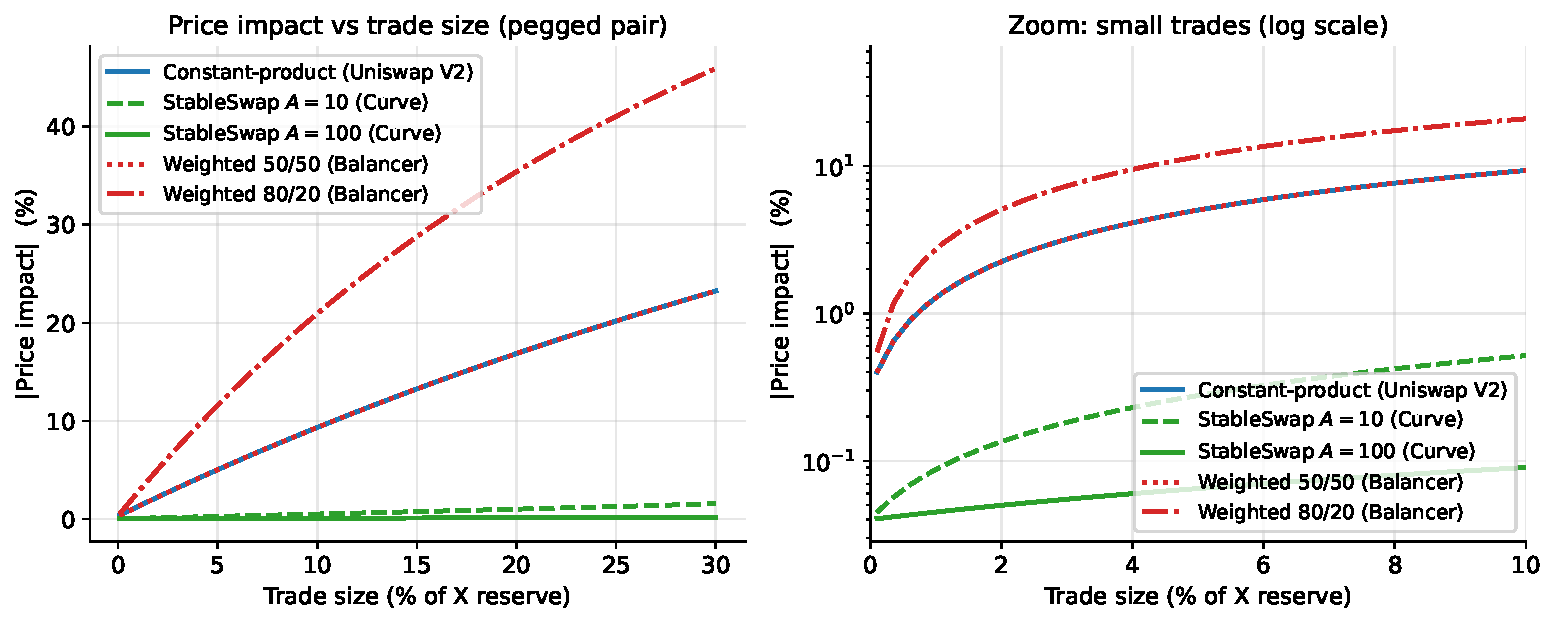
\includegraphics[width=0.97\linewidth]{figures/fig_price_impact.pdf}
\caption{錨定資產對的價格衝擊對比（spot price 皆為 1）。（左）線性座標；（右）對數座標放大小額交易區。StableSwap 的 $A$ 把錨點附近滑點壓到極低，但大額交易會把它推向 constant-product 分支。}
\label{fig:impact}
\end{figure}

\begin{table}[H]\centering\small
\caption{不同情境下的滑點定性排序（「$\ll$」表示顯著較低）。}
\label{tab:sliporder}
\begin{tabularx}{\linewidth}{l l X}
\toprule
資產類型 & 交易規模 & 滑點由低到高（概略） \\
\midrule
錨定（穩定幣） & 小額 & Curve StableSwap $\ll$ 調校過的 Balancer $\sim$ Constant-product；窄區間 V3 可逼近 Curve \\
錨定（穩定幣） & 大額 & Curve 僅在近平衡時最佳；夠大的交易把它推上 constant-product 分支，滑點\emph{可能超過} Uniswap；V3 在區間邊緣有斷崖 \\
波動對 & 小額 & V3（區間內）$<$ V2 全區間；StableSwap 不適用（會嚴重失衡） \\
波動對 & 大額 & 全區間 constant-product 最穩健（無斷崖、平滑凸增）；V3 區間內最便宜但出區間後變差 \\
\bottomrule
\end{tabularx}
\end{table}

% =====================================================================
\section{橫向比較二：LP 收益、無常損失與 LVR}\label{sec:il}
% =====================================================================
\subsection{無常損失與 LP 損益分解}
無常損失（亦稱 divergence loss / loss-versus-holding）衡量 LP 部位相對於單純持有初始資產的相對短缺 \citep{pintailgooddeal,pintailreturns}。50/50 constant-product 的閉式解為 \eqref{eq:v2il}，
其數值見表~\ref{tab:il}。LP 相對 HODL 的淨損益是\emph{累積手續費}與\emph{（負的）無常損失}之和：
\begin{equation}\label{eq:pnl}
\mathrm{PnL}_{\text{LP}}=\underbrace{F}_{\text{手續費}}+\underbrace{\IL(r)\cdot V_{\text{hold}}}_{\le 0},
\qquad\text{LP 勝過持有}\iff \frac{F}{V_{\text{hold}}}\ge 1-\frac{2\sqrt{r}}{1+r}.
\end{equation}
亦即\textbf{手續費必須跑贏無常損失}。圖~\ref{fig:ilpnl}（左）疊出不同手續費收入水準下的淨損益曲線：費用越高、損益曲線越往上抬，使 LP 在更大的價格變動範圍內仍獲利。在有手續費時，套利者的可萃取利潤（與 LP 的逆選擇成本）會被進一步壓低，相關分析見 \citet{milionis2023fees}。

\begin{table}[H]\centering\small
\caption{無常損失隨價格比 $r$ 的變化（單位：\%）。Curve（pegged）在錨點附近近乎為 0。}
\label{tab:il}
\begin{tabular}{lcccccc}
\toprule
價格比 $r=P'/P$ & 1.25 & 1.5 & 2 & 3 & 4 & 5 \\
\midrule
Constant-product 50/50 & $-0.62$ & $-2.02$ & $-5.72$ & $-13.40$ & $-20.00$ & $-25.46$ \\
Balancer 80/20（變動資產 $w{=}0.8$） & $-0.38$ & $-1.20$ & $-3.27$ & $-7.38$ & $-10.84$ & $-13.72$ \\
Balancer 98/2（變動資產 $w{=}0.98$） & $-0.05$ & $-0.14$ & $-0.38$ & $-0.85$ & $-1.25$ & $-1.59$ \\
\bottomrule
\end{tabular}

\end{table}

\begin{figure}[H]
\centering
\begin{subfigure}{0.49\linewidth}\centering
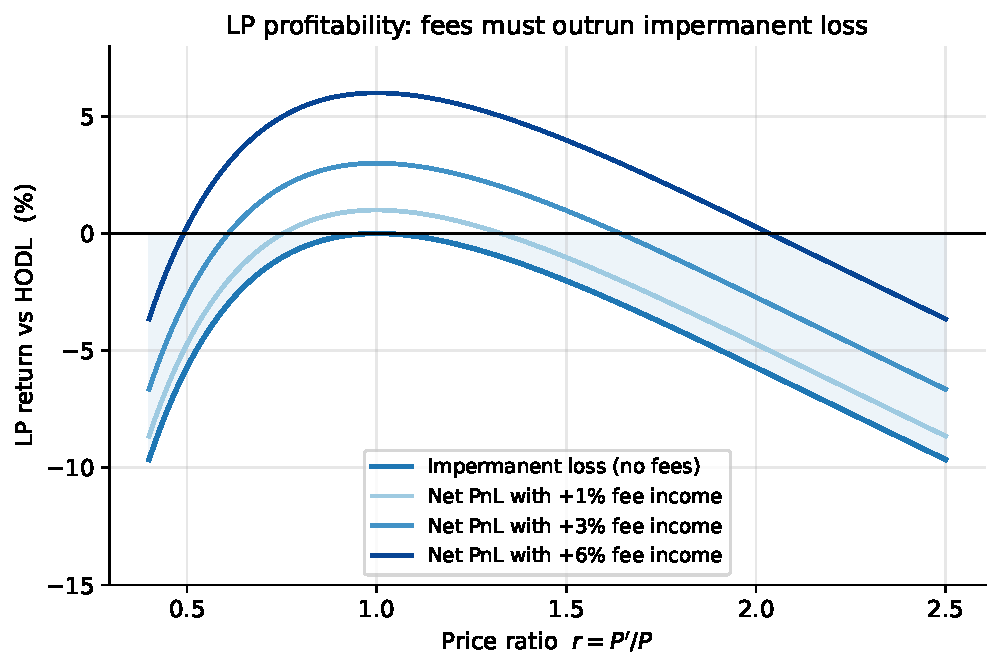
\includegraphics[width=\linewidth]{figures/fig_lp_pnl.pdf}
\caption{LP 淨損益 $=$ 手續費 $-$ 無常損失}
\end{subfigure}\hfill
\begin{subfigure}{0.49\linewidth}\centering
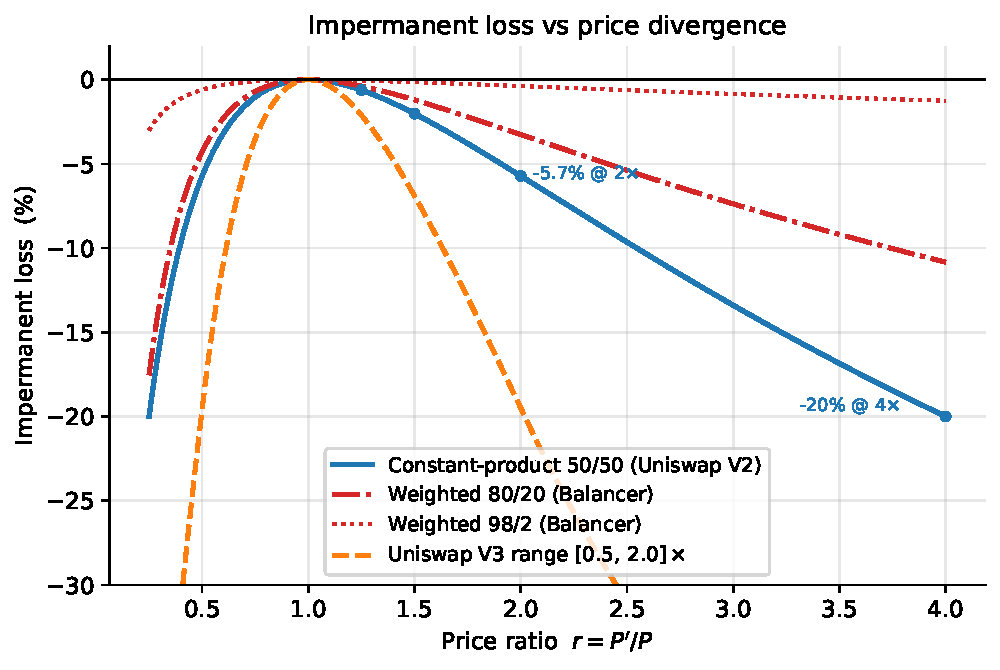
\includegraphics[width=\linewidth]{figures/fig_il_curves.pdf}
\caption{各機制無常損失曲線}
\end{subfigure}
\caption{（a）手續費收入越高，LP 在更寬的價格變動下仍勝過 HODL。（b）無常損失隨價格偏離的比較：constant-product $>$ Balancer 80/20 $>$ 98/2；窄區間 V3 因放大效應最嚴重。}
\label{fig:ilpnl}
\end{figure}

\subsection{Loss-Versus-Rebalancing（LVR）}
傳統無常損失是\emph{路徑無關}的終端量：若價格繞一圈回到起點，IL 歸零。但這掩蓋了一個事實——LP 在過程中持續被套利者「撿便宜」。
\citet{milionis2022lvr} 提出的 \textbf{Loss-Versus-Rebalancing（LVR）}把 LP 成本重新定義為：相對於一個\emph{持續以真實市價再平衡}的參考組合，套利者從 AMM 過時報價中萃取價值的速率。
在波動率為 $\sigma$ 的幾何布朗運動下，瞬時 LVR 率為
\begin{equation}\label{eq:lvr}
\ell(\sigma,P)=\tfrac12\,\sigma^2 P^2\,\bigl|x'(P)\bigr|=-\tfrac12\,\sigma^2 P^2\,V''(P),
\end{equation}
與波動率\emph{平方}、邊際流動性（價值函數的二階導）成正比。對 constant-product 這收斂為著名的價格無關常數
\begin{equation}
\frac{\ell}{V(P)}=\frac{\sigma^2}{8},\qquad\text{加權池}\quad \frac{\ell}{V(P)}=\frac{\sigma^2}{2}w(1-w).
\end{equation}
故 80/20 池（$w(1-w)=0.16$）的 LVR 較 50/50（$0.25$）少約 $36\%$。累積 LVR 恰為「邊際流動性加權的變異數交換（variance swap）」的浮動腿，凸顯出\emph{是已實現變異數、而非淨位移}在侵蝕 LP 價值。會計恆等式為
\begin{equation}
V^{\text{LP}}_T=V^{\text{rebalance}}_T-\mathrm{LVR}_{[0,T]}+F_T .
\end{equation}

\keybox{\textbf{IL 與 LVR 的關鍵差異}：IL 是\emph{路徑無關、終端}的（價格回到起點即歸零）；LVR 是\emph{單調遞增、逐筆累積}給套利者／MEV 的\emph{連續成本}，只要價格路徑有非零變異數就嚴格為正——即使在 IL 為零的來回行情中亦然。LVR 因此是 AMM 造市的真實逆選擇成本，也是 v4 動態費率與批次／拍賣型 AMM 想解決的核心。}

各機制 IL/LVR 由\emph{曲率與權重}決定，排序為：Curve（近錨點）$\approx$ Balancer 高權重資產 $<$ Balancer 80/20 $<$ Uniswap V2 50/50 $<$ 窄區間 Uniswap V3（放大最劇）。

% =====================================================================
\section{情境模擬：不同波動率與交易量下的 LP 報酬}\label{sec:mc}
% =====================================================================
為直接回應題目「\emph{模擬不同流動性與交易量情境}」，本節以\textbf{蒙地卡羅}量化各機制 LP 相對 HODL 的報酬分佈。

\paragraph{模型設定。} 風險資產 X 相對計價資產 Y 服從無漂移的幾何布朗運動（年化波動率 $\sigma$）。套利者持續把每個池的邊際價格拉回外部市價，故池子的準備金價值是價格比 $r=P_t/P_0$ 的確定函數
$\mathrm{PV}(r)$（閉式：constant-product $\sqrt{r}$；權重 $w$ 池 $r^{w}$；V3 由 \eqref{eq:v3reserves} 之虛擬準備金導出）。手續費以「年化成交量 $=$ \texttt{turnover}$\times$TVL」逐日累計；
V3 集中部位在區間內賺取 $E$ 倍手續費（資本效率，\eqref{eq:v3eff}）、出區間則為零。LP 相對 HODL 的報酬為
\[
\text{LP-vs-HODL}=\frac{\mathrm{PV}(r_T)+\text{累積手續費}}{V_{\text{hold}}(r_T)}-1 .
\]
每個情境模擬 $5000$ 條一年期路徑（每日步進、手續費率 $0.3\%$）。

\paragraph{結果。} 圖~\ref{fig:mc} 與表~\ref{tab:mc} 呈現結果。可觀察到清楚的結構：
\begin{itemize}
  \item \textbf{Uniswap V3} 在\emph{低波動 $+$ 高量}時報酬最高（集中流動性使手續費被放大 $\approx 3.4\times$，且價格多停留在區間內）；但在\emph{高波動}時最差——無常損失被放大、且價格易跌出 $[0.5,2]$ 區間而停止收費（$\sigma{=}150\%$、量 $10\times$ 時平均 $-40.7\%$）。
  \item \textbf{Balancer 98/2} 最接近 HODL：無常損失極小，報酬最穩健，在高波動下仍多為正。
  \item \textbf{成交量（流動性使用率）}是 LP 能否勝過 HODL 的關鍵：右圖顯示量從 $10\times$ 升到 $200\times$，所有機制「勝過 HODL 的機率」都大幅上升並趨近 100\%。
\end{itemize}
這從模擬層面印證了 \eqref{eq:pnl}：\textbf{手續費必須跑贏無常損失}，而手續費由成交量驅動、無常損失由波動率驅動。

\begin{figure}[H]
\centering
\begin{subfigure}{0.46\linewidth}\centering
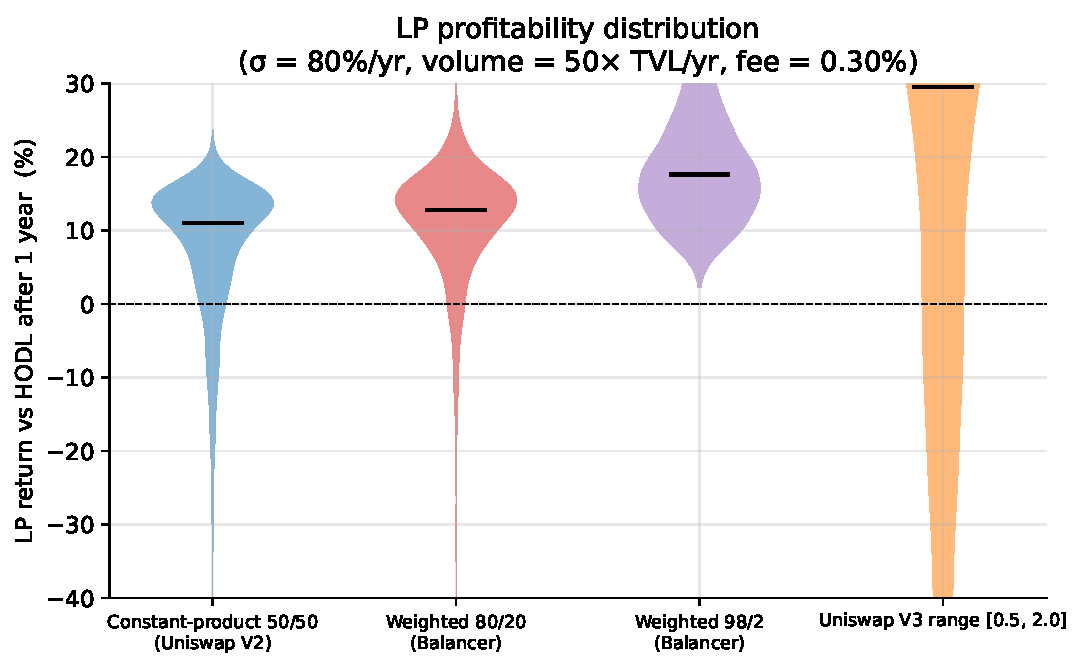
\includegraphics[width=\linewidth]{figures/fig_mc_distributions.pdf}
\caption{報酬分佈（$\sigma{=}80\%$、量 $50\times$）}
\end{subfigure}\hfill
\begin{subfigure}{0.52\linewidth}\centering
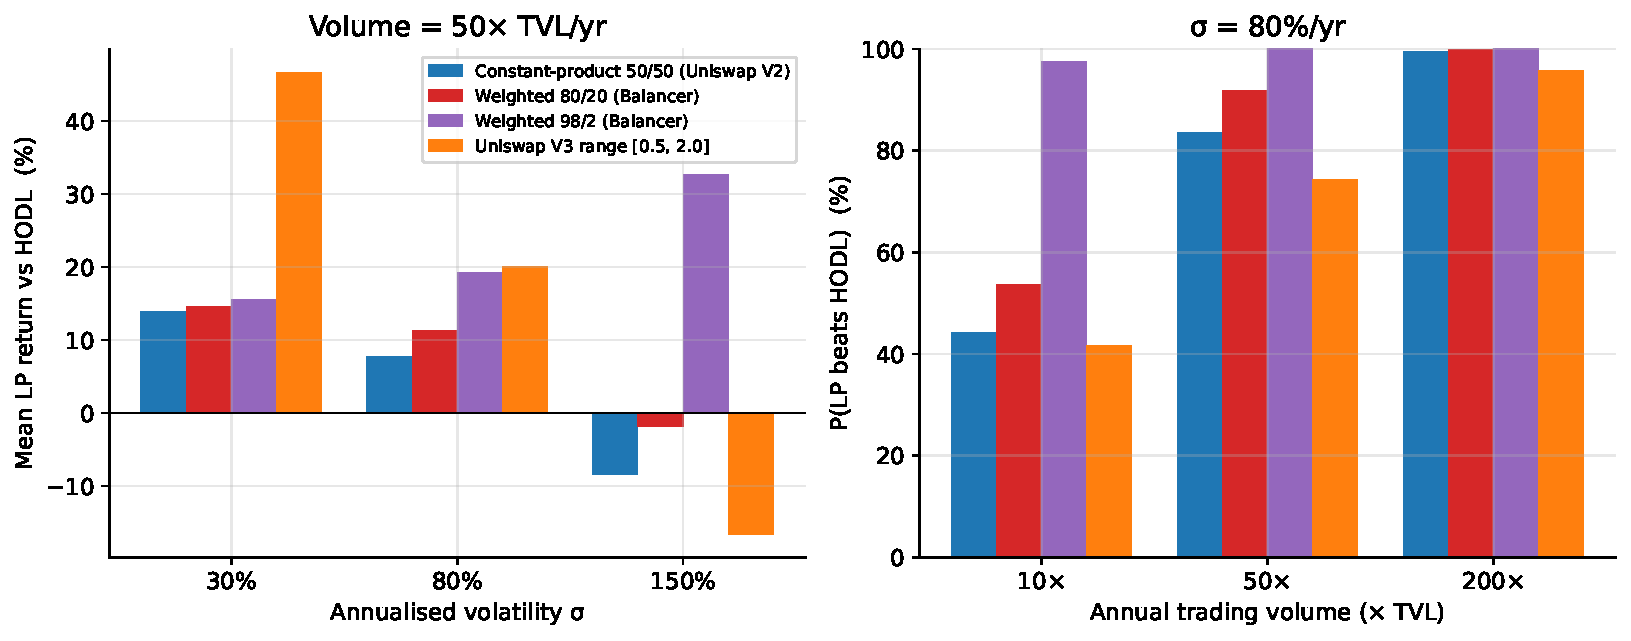
\includegraphics[width=\linewidth]{figures/fig_mc_scenarios.pdf}
\caption{跨波動率／交易量情境}
\end{subfigure}
\caption{蒙地卡羅模擬 LP 相對 HODL 的一年期報酬。（a）小提琴圖顯示各機制的報酬分佈與中位數；（b）左：平均報酬隨波動率變化（量固定 $50\times$）；右：勝過 HODL 的機率隨成交量上升。}
\label{fig:mc}
\end{figure}

\begin{table}[H]\centering\small
\caption{蒙地卡羅情境結果：各機制 LP 相對 HODL 的\emph{平均}報酬，以及 50/50 池勝過 HODL 的機率。}
\label{tab:mc}
\begin{tabular}{cc|cccc}
\toprule
$\sigma$ (年化) & 年成交量 & \multicolumn{4}{c}{LP 相對 HODL 的平均報酬與勝率} \\
 & ($\times$TVL) & 50/50 & 80/20 & V3[0.5,2] & $P(\text{50/50}{>}0)$ \\
\midrule
30\% & 10$\times$ & +1.9\% & +2.3\% & +6.3\% & 90\% \\
30\% & 50$\times$ & +13.9\% & +14.6\% & +46.7\% & 100\% \\
30\% & 200$\times$ & +59.1\% & +60.6\% & +198.3\% & 100\% \\
80\% & 10$\times$ & -4.5\% & -2.6\% & -12.7\% & 44\% \\
80\% & 50$\times$ & +7.8\% & +11.3\% & +20.1\% & 83\% \\
80\% & 200$\times$ & +54.0\% & +63.3\% & +143.0\% & 99\% \\
150\% & 10$\times$ & -21.0\% & -18.9\% & -40.7\% & 21\% \\
150\% & 50$\times$ & -8.5\% & -1.8\% & -16.6\% & 47\% \\
150\% & 200$\times$ & +38.7\% & +62.5\% & +73.7\% & 88\% \\
\bottomrule
\end{tabular}
\end{table}

% =====================================================================
\section{綜合比較與設計取捨}\label{sec:compare}
% =====================================================================
表~\ref{tab:matrix} 彙整三大家族在八個維度上的差異。整體而言，\emph{沒有最好的 AMM，只有最適合特定資產與目標的 AMM}。

\begin{table}[H]\centering\footnotesize
\caption{Constant-Product、Stable-Swap 與 Weighted-Pool 綜合比較矩陣。}
\label{tab:matrix}
\renewcommand{\arraystretch}{1.35}
\begin{tabularx}{\linewidth}{p{2.3cm} X X X}
\toprule
維度 & \textbf{Constant-Product}（Uniswap V2/V3） & \textbf{Stable-Swap}（Curve） & \textbf{Weighted-Pool}（Balancer）\\
\midrule
不變量 & $xy=k$（V3 在 tick 區間內以虛擬準備金 $L^2=xy$） & $An^n\!\sum x_i+D=ADn^n+\frac{D^{n+1}}{n^n\prod x_i}$（混合和與積） & $V=\prod_t B_t^{W_t},\ \sum W_t=1$（幾何平均）\\
邊際價格 & $p=y/x$；手續費以 $\gamma=0.997$ 平移 & 錨點附近 $\approx 1$（平坦）；脫錨後回到 $y/x$ 型態 & $SP=\frac{B_i/W_i}{B_o/W_o}$；費用乘上 $1/(1-f)$\\
滑點曲線 & 凸；小額近線性、不可抽乾 & 近錨點近零（深度 $\sim A\!\cdot\!R$）；脫錨成斷崖 & 由 $W_i/W_o$ 縮放；高權重幣同 TVL 下滑點更低\\
資本效率 & V2 全區間（低）；V3 集中可達 $\sim4000\times$ & 錨點附近高（$A$ 倍局部深度） & 同 V2（全區間）；80/20 把深度偏向高權重幣\\
無常損失 & $\IL=\frac{2\sqrt r}{1+r}-1$；$2\times$ 為 $-5.72\%$；V3 區間內放大 & pegged 極小，僅脫錨時顯著 & $\IL=\frac{r^w}{wr+1-w}-1$；80/20 較 50/50 少約 $43\%$\\
手續費 & V2 0.3\% 複利進 $k$；V3 分級 $0.01/0.05/0.3/1\%$、不複利 & 低（$\sim0.04$--$0.06\%$）；V2 動態費率隨失衡上升 & 單一可設定費率 $f$，以 $(1-f)A_i$ 代入\\
適用場景 & V2 長尾任意對；V3 想要集中、資本效率的主動 LP & 互相錨定／高相關資產（穩定幣、LST） & 多資產指數池、80/20 協議自有流動性、LBP 發行\\
主要風險 & 無常損失與 LVR；V3 另有出區間失效與管理負擔 & 脫錨風險（LP 吸收壞資產）；脫錨後滑點可能超過 product 池 & 仍有 IL/LVR；高權重與 LBP 池集中單一資產風險\\
\bottomrule
\end{tabularx}
\end{table}

圖~\ref{fig:designspace} 把三者放在「資產相關性 $\times$ 資本效率／管理成本」的設計空間中，給出直觀的選型地圖。

\begin{figure}[H]
\centering
\resizebox{\linewidth}{!}{%
\begin{tikzpicture}[font=\small,>=Stealth]
% axes
\draw[->,thick] (0,0) -- (11,0) node[below right]{資產相關性 / 錨定程度 $\rightarrow$};
\draw[->,thick] (0,0) -- (0,6.6) node[above left]{資本效率 / 主動管理需求 $\rightarrow$};
\node[align=center,font=\scriptsize] at (1.7,-0.55) {波動、不相關\\(ETH/長尾)};
\node[align=center,font=\scriptsize] at (9.2,-0.55) {高度錨定\\(USDC/USDT)};
% regions / markers
\node[draw,rounded corners,fill=blue!8,align=center,minimum width=2.6cm] (v2) at (2.2,1.5)
  {\textbf{Uniswap V2}\\ $xy=k$\\ \scriptsize 通用、被動};
\node[draw,rounded corners,fill=blue!14,align=center,minimum width=2.6cm] (v3) at (2.6,4.7)
  {\textbf{Uniswap V3}\\ 集中流動性\\ \scriptsize 高效率、需主動管理};
\node[draw,rounded corners,fill=red!10,align=center,minimum width=2.6cm] (bal) at (5.7,2.6)
  {\textbf{Balancer}\\ 加權 / 80/20 / LBP\\ \scriptsize 多資產、指數};
\node[draw,rounded corners,fill=green!12,align=center,minimum width=2.6cm] (curve) at (9.0,2.0)
  {\textbf{Curve StableSwap}\\ 放大係數 $A$\\ \scriptsize 錨定資產近零滑點};
\node[draw,rounded corners,fill=green!18,align=center,minimum width=2.6cm] (cv2) at (8.4,4.8)
  {\textbf{Curve V2}\\ 動態錨定\\ \scriptsize 波動對、自動集中};
\draw[->,dashed,gray] (v2) -- (v3) node[midway,right,font=\scriptsize,gray]{集中};
\draw[->,dashed,gray] (curve) -- (cv2) node[midway,right,font=\scriptsize,gray]{動態錨定};
\end{tikzpicture}%
}
\caption{AMM 設計空間定位圖。橫軸為資產錨定程度，縱軸為資本效率／主動管理需求。三大家族各佔不同區位，V3 與 Curve V2 分別是 V2 與 StableSwap 朝「高資本效率」方向的演化。}
\label{fig:designspace}
\end{figure}

\paragraph{選型指南。}
\begin{itemize}
  \item \textbf{穩定幣 / LST（如 USDC--USDT、stETH--ETH）}：選 Curve StableSwap——錨點附近近零滑點且無常損失極小。
  \item \textbf{波動主流對（如 ETH--USDC）}：選 Uniswap V3（主動管理區間以追求資本效率）或 V2（被動、省心）。
  \item \textbf{多資產配置 / 協議自有流動性 / 代幣公平發行}：選 Balancer 指數池、80/20 或 LBP。
  \item \textbf{波動且不錨定的多元資產（如 ETH/BTC/USD）}：選 Curve V2 CryptoSwap——免人工管理區間即得集中流動性。
\end{itemize}

% =====================================================================
\section{前沿發展（額外內容）}\label{sec:frontier}
% =====================================================================
\paragraph{Uniswap v4：把 AMM 變成可程式化平台。}
v4 \citep{uniswapv4wp,uniswapv4vision,uniswapv4hooks} 不改變 V3 的集中流動性核心，而是圍繞四個擴充原語重構：
\textbf{(1) Hooks}——外部合約在池子生命週期的指定時點被回呼，v4 定義\emph{恰好十個}回呼（before/after $\times$ Initialize、AddLiquidity、RemoveLiquidity、Swap、Donate）；hook 合約\emph{位址}本身編碼啟用哪些回呼。
hooks 可原生實作動態（波動率）費率、TWAMM、鏈上限價單、自訂預言機，甚至以 Custom Accounting 繞過集中流動性曲線實作任意曲線（如 v2 式 $xy=k$）。
\textbf{(2) Singleton}：所有池放在單一合約，建池 gas 降約 $99\%$、多跳交換更便宜。\textbf{(3) Flash accounting}：交易期間只記錄淨額（delta），結束時以 \texttt{take()/settle()} 強制償付（EIP-1153 transient storage）。\textbf{(4) ERC-6909} 多代幣記帳並恢復原生 ETH 支援。

\paragraph{LVR / MEV 緩解型 AMM。}
LVR \citep{milionis2022lvr,a16zlvr} 被視為比搶跑與三明治攻擊加總更大的 MEV 來源，催生數種新設計：
\textbf{FM-AMM}（function-maximizing AMM）\citep{canidio2023fmamm} 把整個區塊的交易\emph{批次}以單一統一清算價成交，使競爭的套利者把價格推到外部市價，消除 LVR 式套利租金與三明治攻擊；
\textbf{CoW AMM}（CoW Protocol，2024 上線於 Balancer）\citep{cowammdocs,cowammlaunch} 是其生產化——求解者（solver）在批次拍賣中競爭，出價對池子\emph{剩餘最多}者贏得再平衡權，把套利價值還給 LP（首個「MEV-capturing AMM」）；
\textbf{am-AMM}（auction-managed AMM）\citep{adams2024amamm} 則以抗審查的鏈上拍賣出售暫時的「池子經理人」角色，由其設定費率並收取全部手續費以內部化小幅價格變動套利，在其假設下可維持高於任何固定費率 AMM 的均衡流動性，並被列為候選 v4 hook。

\paragraph{動態費率與 JIT 流動性。}
\textbf{即時（Just-in-time, JIT）流動性} \citep{uniswapjit,jitaft2025} 是集中流動性下的 MEV 策略：LP 看到 mempool 中即將到來的大額交易，於其前鑄造極窄區間部位、其後立刻銷毀，攫取該筆交易幾乎全部手續費並稀釋被動 LP（研究指對被鎖定交易稀釋可達約 $85\%$）。
v4 原生的動態費率 hook 是一種防禦：在波動／有毒流期間提高費率以補償被動 LP 的 LVR。

\paragraph{真實市場規模（約 2025--2026 快照，數值會波動）。}
依 DefiLlama \citep{defillamauniswap,defillamacurve,defillamabalancer}，Uniswap 為最大 DEX，整合 TVL 約數十億美元等級、30 日 DEX 交易量達數百億美元級；v4 於 2025 年初上線後約 177 天達到約 \$1B TVL。
Curve TVL 約 \$1.4B（多在以太坊），Balancer 約 \$100--130M，規模遠小於前兩者。此數據佐證了設計取捨在市場上的回響：通用的 Uniswap 取得最大份額，Curve 在穩定幣利基穩固，Balancer 則服務於指數／發行等專門需求。

% =====================================================================
\section{結論}
% =====================================================================
本報告在 CFMM 統一框架下，完整推導並比較了 Constant-Product、Stable-Swap 與 Weighted-Pool 三大 AMM 家族的數學模型與核心機制，並以理論與蒙地卡羅模擬量化其滑點、LP 收益與無常損失差異。核心結論為：

\begin{enumerate}
  \item \textbf{三者本質皆為 CFMM}，差別只在交易函數 $\varphi$：Uniswap 用 $xy=k$、Balancer 用加權幾何平均、Curve 用以放大係數 $A$ 調控的「和--積」混合。
  \item \textbf{滑點服從單一規則} $\text{slippage}\approx\Delta x/(2\mathcal{D})$；局部深度 $\mathcal{D}$ 可被 Curve 的 $A$、V3 的集中度 $L$、或 Balancer 的權重放大——這是三者差異的統一解釋。
  \item \textbf{無常損失是價格比的函數}；Balancer 加權可降低之，Curve 對 pegged 資產近乎為零，而 V3 集中流動性以\emph{放大無常損失}換取資本效率。
  \item \textbf{LVR} 提供比傳統 IL 更貼近真實的造市成本視角，並驅動了 v4 動態費率與批次／拍賣型 AMM 等前沿設計。
  \item \textbf{模擬證實}手續費（由成交量驅動）必須跑贏無常損失（由波動率驅動）；故「最佳 AMM」取決於資產特性與 LP 目標，而非單一冠軍。
\end{enumerate}

所有公式皆以多代理（multi-agent）survey 對照一手白皮書與學術論文，並經對抗式驗證（過程中修正了 V3 tick 公式底數與 Curve V2 repegging 係數兩處）；圖表與數據由附錄所述之 Python 程式完全重現。

% =====================================================================
\section*{附錄：模擬方法與可重現性}
\addcontentsline{toc}{section}{附錄：模擬方法與可重現性}
% =====================================================================
所有圖表由本專案 \texttt{sim/} 目錄下之 Python 程式產生（相依 \texttt{numpy/scipy/matplotlib}）：
\begin{itemize}\setlength{\itemsep}{1pt}
  \item \texttt{amm.py}：三種 AMM 池的參考實作（含以 \texttt{scipy.brentq} 求解 StableSwap 不變量），與無常損失／資本效率閉式解。
  \item \texttt{make\_figures.py}：產生鍵結曲線、價格衝擊、無常損失、V3 資本效率、StableSwap 放大係數、LP 損益等解析圖（圖~\ref{fig:bonding}--\ref{fig:ilpnl}）。
  \item \texttt{simulate\_lp.py}：第~\ref{sec:mc} 節之蒙地卡羅模擬，輸出報酬分佈、情境圖與表~\ref{tab:mc}。
\end{itemize}
本報告所用之三種 AMM 自我檢驗（範例）：$x{=}y{=}1000$、輸入 100 時，Constant-product 產出 $90.66$（滑點明顯），StableSwap（$A{=}100$）產出 $99.91$（近 1:1），印證放大係數對滑點的壓制。

\medskip\noindent\textbf{完整原始碼}（LaTeX、Python 模擬與圖表）公開於 GitHub：\\
\url{https://github.com/ZhenXiang6/amm-mechanisms-comparison}

% ---------- 參考文獻 ----------
\bibliographystyle{plainnat}
\bibliography{refs}

\end{document}
